\section{Results}

The current experiments investigate the influence of fixation type and associated eye movements on the perception of self-motion. Participants were presented with two subsequent lateral translations (\figref{p3:fig1}) and they had to judge whether the second was longer or shorter than the first. During each interval participants fixated a body- or world-fixed target (body and world fixation) or were moved in absence of a fixation point (free fixation).

\begin{figure}
    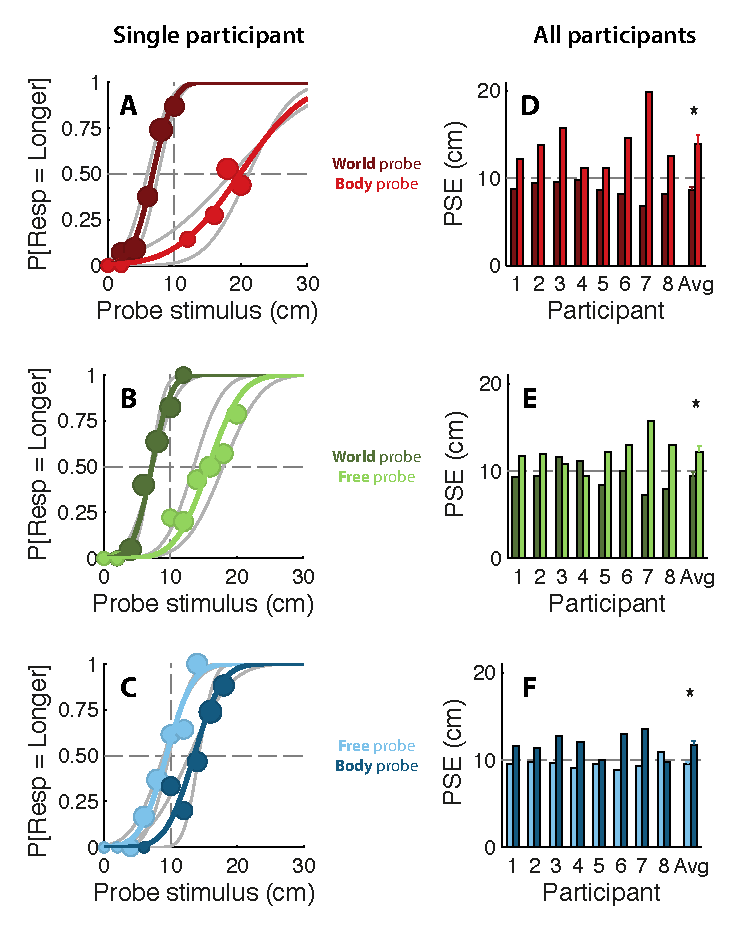
\includegraphics[width=1.0\textwidth]{src/paper3/figure2.pdf}

    \caption{Psychometric curves (colored lines) and associated binned data (circles) for one participant (top row). Circle size represents the number of trials within each 2 \si{\centi\metre} bin. Binning was only done in order to visualize this participant's responses and was not used otherwise. Gray lines show psychometric curves before collapsing across reference order. \panelref{A} Body-world comparison; body reference, dark red; world reference, light red. \panelref{B} World-free comparison; world reference, light green; free reference, dark green. \panelref{C}  Body-free comparison; body reference, dark blue; free reference, light blue. \newline
PSEs for all participants and the average {\textpm}SE (bottom row). \panelref{D} Body-world (dark red) and world-body (light red) conditions. \panelref{E} World-free (light green) and free-world (dark green) conditions. \panelref{F} Body-free (dark blue) and free-body (light blue) conditions. Because a t-test revealed a main effect of reference order, \ttest{47}{-5.2}{0.01}, we used the mean PSE across reference order (e.g. \figref{p3:fig3}, gray lines) instead of the PSE collapsing across reference order (e.g. \figref{p3:fig3}, colored lines); these values were not significantly different.}
    \label{p3:fig2}
\end{figure}

The performance of one participant is illustrated in the left column of \figref{p3:fig2}. Each row shows one main condition: body versus world fixation (top/red), world versus free fixation (middle/green), and body versus free fixation (bottom/blue). The lighter and darker colors in each panel indicate which fixation type was the reference movement (see Legend). The shift of the psychometric functions relative to the 10 \si{\centi\metre} reference (i.e. the PSE) quantifies the influence of fixation type. For example, the rightward shift of the light red curve in \figref{p3:fig2}A means that for a body fixation a longer translation (\about 19 \si{\centi\metre}) was required for that translation to be perceived equivalent to a 10\si{\centi\metre} reference translation with world fixation. On the other hand, the leftward shift of the dark red curve means that a shorter translation with world fixation (\about 7 \si{\centi\metre}) was required for that translation to be perceived equivalent to the 10 \si{\centi\metre} reference translation with body fixation. Together, these oppositely directed shifts demonstrate that translations with world fixation were perceived longer than equivalent translations with body fixation, regardless of which translation was the reference.  Similarly, the shifts in \figref{p3:fig2}B shows that world fixation translations were also perceived to be longer than free fixation movements and \figref{p3:fig2}C shows that free fixation translations were perceived to be longer than body fixation translations. Note that \figref{p3:fig2} also shows effects on slope, which will be further discussed in the paragraph \nameref{p3:sec:precision}.

Similar results were obtained for all subjects, as shown by the individual PSEs for all participants (right column of \figref{p3:fig2}). Statistical significance of the fixation-induced effects for each main condition (world versus body, \figref{p3:fig2}D; world versus free, \figref{p3:fig2}E; and free versus body, \figref{p3:fig2}F) was evaluated by comparing PSEs between the two reference conditions using a paired t-test. These PSEs were significantly different in all cases (world versus body, \ttest{7}{-4.09}{0.05}; world versus free, \ttest{7}{-2.48}{0.05}; free versus body, \ttest{7}{-3.38}{0.05}. As for the example subject, these results indicate that translations made with body fixation are perceived shorter than with world fixation, suggesting that self-motion perception is modulated by eye movements even in absence of full-field optic flow. The free fixation translations, which control for confounds of the small fixation point, were perceived to be longer than body and shorter than world fixation translation intervals, which could be expected if their gains were smaller than 1 but larger than 0.

\begin{figure}
    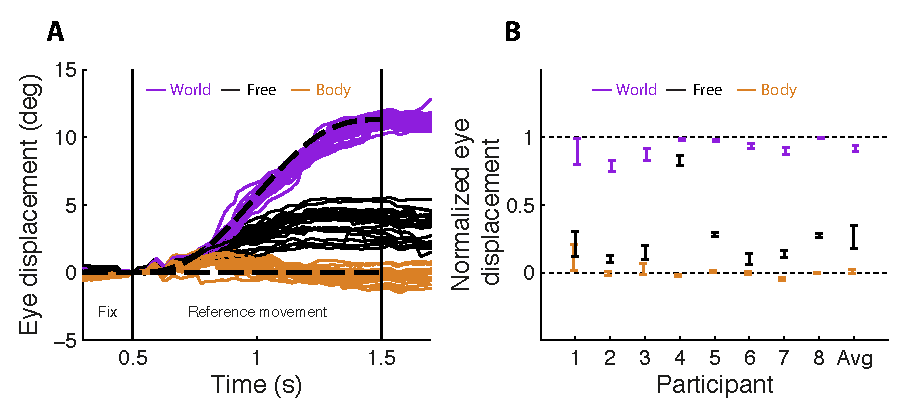
\includegraphics[width=1.0\textwidth]{src/paper3/figure3.pdf}

    \caption{\panelref{A} Actual (solid lines) and ideal (dashed lines) eye movement traces of one participant during world fixation (purple), body fixation (brown), and free fixation (black). All traces shown are for 10 \si{\centi\metre} reference movements. \panelref{B} Normalized eye position for each participant (\textpm95\% confidence interval) at the end of translation interval (error bars) for world fixation (purple), body fixation (brown) and free fixation (blue). In addition, the average {\textpm}SE across all participants is shown. Zero indicates that the eyes remained stationary relative to the body, and one indicates that eye position was perfectly world-fixed.}
    \label{p3:fig3}
\end{figure}

\subsection{Eye movement contributions to self-motion perception}

In order to relate psychophysical performance to eye movement behavior we recorded and analyzed eye movements during both intervals of every trial for all subjects. Exemplar eye traces for the 10 \si{\centi\metre} reference translation for the three fixation types are depicted in \figref{p3:fig3}A. Fixation behavior was quite accurate for both body fixations, where no eye movements were expected, and world fixation, where eye movement excursions of \siang{11} were expected, seemingly supported by  catch-up saccades. Under free fixation, the amount of eye movement was intermediate between body and world fixation and behavior was more variable. A similar pattern was observed in all participants, as illustrated by the normalized eye movement data (see \nameref{p3:sec:methods}, and \figref{p3:fig3}B).

\begin{figure}
    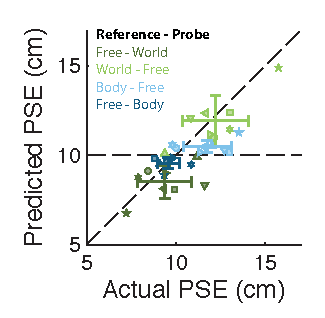
\includegraphics[width=0.5\textwidth]{src/paper3/figure4.pdf}

    \caption{Eye movement based prediction for the PSE plotted against the actual PSE.  A data point (symbol) is shown for each participant (symbol shape) and condition (symbol color) pair, following the same color scheme as in \figref{p3:fig2}. The identity line, corresponding to a perfect prediction, is shown in black.}
    \label{p3:fig4}
\end{figure}

\begin{table}
    \begin{tabular}{llll}
    Participant & Parameter ($\alpha$) \textpm SD \\
    \hline
    1 & 0.27 (\textpm 0.04) \\
    2 & 0.27 (\textpm 0.05) \\
    3 & 0.35 (\textpm 0.04) \\
    4 & 0.06 (\textpm 0.04) \\
    5 & 0.13 (\textpm 0.03) \\
    6 & 0.33 (\textpm 0.04) \\
    7 & 0.58 (\textpm 0.02) \\
    8 & 0.21 (\textpm 0.02) \\    
    \end{tabular}
    
    \caption{Estimated eye movement contribution (α) to the perception of self-motion (see Equation 5). Standard deviations are based on a bootstrap for each participant.}
    
    \label{p3:tab2}
\end{table}

To quantify the role of eye movements in self-motion perception, we tested a linear model (see \nameref{p3:sec:model}) in which perceived translation is a weighted average of a vestibular estimate (equal to the actual translation) and an oculomotor estimate (equal to the normalized eye movement times the actual translation; \eqnref{p3:eq2}). This model contains a single free parameter ($\alpha$), which corresponds to the relative weight given to the oculomotor estimate. We fit this model to the two body versus world conditions and obtained the value of the oculomotor weight for every subject (\tabref{p3:tab2}). The average oculomotor weight is 0.25 \textpm0.12 (SD), indicating that the contribution of the eye movement signal to the self-motion estimate is about 25 percent. Note that participant 4, whose oculomotor weight is furthest from this mean ($\alpha = 0.06$), also shows a radically different eye movement gain during the free-fixation (see \figref{p3:fig3}B). We then used these oculomotor weights along with the normalized eye movement values to predict the PSEs in the remaining four conditions according to \eqnref{p3:eq5}. The predicted PSEs are plotted against the actually observed PSEs in \figref{p3:fig4}. The positive correlation ($\rho = 0.78$, $p < 0.01$) between observed and predicted PSEs suggests that eye movements are indeed used in self-motion perception, even in the absence of a fixation point (i.e. during free fixation). Furthermore, the fact that data points generally cluster near the unity line shows that our simple model does reasonably well in predicting perceptual performance across subjects and conditions based on oculomotor weight and normalized eye movement magnitude only. This holds true even for subject 7 whose oculomotor weight (\tabref{p3:tab2}) was approximately double the average, yet whose data points remain close to the unity line.

\begin{figure}
    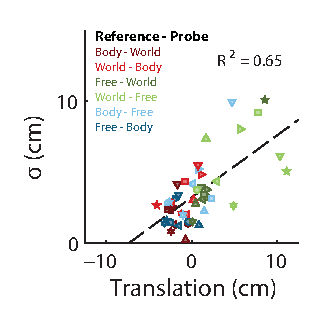
\includegraphics[width=0.5\textwidth]{src/paper3/figure5.pdf}

    \caption{Effect of difference movement amplitude between reference and probe interval (i.e. the bias) on response uncertainty ($\sigma$). A data point is shown for every participant and condition (symbol color) pair, following the same color scheme as in \figref{p3:fig2}. The dashed black line is the linear regression trend line.}
    
    \label{p3:fig5}
\end{figure}

\subsection{Precision depends on PSE}
\label{p3:sec:precision}

The psychometric curves of the example participant in \figref{p3:fig2} show that precision ($\sigma^{-2}$ in \eqnref{p3:eq1}) decreases as the difference between translated distance in the reference and probe intervals (i.e. the bias) increases. In \figref{p3:fig5} precision is plotted as a functions of bias for all participants and all conditions, showing a significant linear relationship ($R^2 = 0.64$) between the two. This effect, which follows Weber's perceptual law \cite{fechner1860} is consistent with the signal-dependence of (discrimination) precision that has been shown recently for vertical self-motion \cite{nesti2014}.

